
%(BEGIN_QUESTION)
% Copyright 2006, Tony R. Kuphaldt, released under the Creative Commons Attribution License (v 1.0)
% This means you may do almost anything with this work of mine, so long as you give me proper credit

En "smart" differansetrykktransmitter er konfigurert for å måle differansetrykket over en orifiseplate, og samtidig utføre kvadratrotfunksjonen som lineariserer signalet:

$$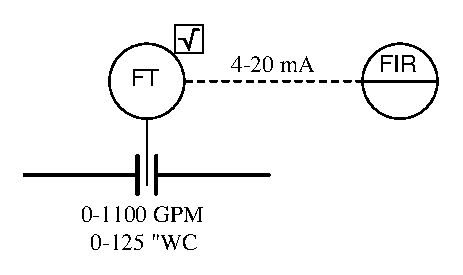
\includegraphics[width=15.5cm]{i00708x01.eps}$$

Beregn følgende:

\begin{itemize}
\item{} Sløyfestrøm ved 350 GPM = \underbar{\hskip 50pt} mA
\vskip 5pt
\item{} Differansetrykk ved 600 GPM = \underbar{\hskip 50pt} "WC
\end{itemize}

\underbar{file i00708no}
%(END_QUESTION)





%(BEGIN_ANSWER)

\begin{itemize}
\item{} Sløyfestrøm ved 350 GPM = \underbar{\bf 9.091} mA
\vskip 5pt
\item{} Differansetrykk ved 600 GPM = \underbar{\bf 37.19} "WC
\end{itemize}

%(END_ANSWER)





%(BEGIN_NOTES)


%INDEX% Måling, flow: orifiseplate sløyfeberegninger

%(END_NOTES)
